% Nallino, Part II p. 251: the inclination of the epicycle of Venus or Mercury, redrawn from the print at the size of
% the print. The coordinates are those of a 400 dpi render of the figure (crop from x 350 pt, y 215 pt of the master
% page; y downward). The epicycle DGAZ has its centre in H; AD and GZ are perpendicular diameters, HE the line to the
% Earth E; T is the planet, K the foot of its perpendicular on AD, N and L the feet of the perpendiculars from T and K
% on the plane of the ecliptic (L on HE). Dashed as on the print: TN, NL, NE and TE. A short stroke crosses HD.
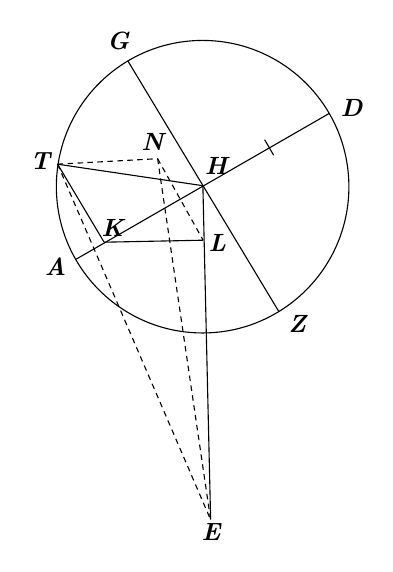
\begin{tikzpicture}[x=0.0635mm,y=-0.0635mm,line width=0.4pt,every node/.style={font=\bfseries\itshape\small,inner sep=1pt}]
\path (50,38);
\coordinate (H) at (396.5,354);
\coordinate (T) at (106,311);
\coordinate (K) at (199,467);
\coordinate (L) at (397,463);
\coordinate (N) at (306,300);
\coordinate (E) at (412,1022);
\draw (396,356) circle[radius=292.5];
\draw (246.5,104.5) -- (548,605);
\draw (143,501) -- (650,209);
\draw (520,262) -- (538,293);
\draw (T) -- (H);
\draw (T) -- (K);
\draw (K) -- (L);
\draw (H) -- (E);
\begin{scope}[dash pattern=on 2pt off 1.6pt]
\draw (T) -- (N);
\draw (N) -- (L);
\draw (N) -- (E);
\draw (T) -- (E);
\end{scope}
\node at (227.5,64.5) {G};
\node at (694,198) {D};
\node at (296,266) {N};
\node at (71.5,305) {T};
\node at (423,314) {H};
\node at (216,438) {K};
\node at (425.5,469) {L};
\node at (101.5,517.5) {A};
\node at (585,629.5) {Z};
\node at (413,1047) {E};
\end{tikzpicture}
